\documentclass{beamer}

\mode<presentation> {
	
	\usetheme{default}
	%\usetheme{Rochester}
	%\usecolortheme{lily}
	
	\setbeamertemplate{footline}[page number] 
	\beamertemplatenavigationsymbolsempty
	\setbeamertemplate{bibliography item}{} %Remove icons in bibliography
}

\usepackage{graphicx} % Allows including images
\usepackage{amsmath}
\usepackage{lmodern}
\usepackage{listings}
\usepackage{hyperref}
\usepackage{wrapfig}



\usepackage{tikz}
\usetikzlibrary{bayesnet}

\lstset{
	language=[5.0]Lua,
	basicstyle=\fontsize{11}{9},
	sensitive=true,
	breaklines=true,
	tabsize=2
}

%----------------------------------------------------------------------------------------
%	TITLE PAGE
%----------------------------------------------------------------------------------------

\title[DEF]{SGVB Topic Modelling} 
\subtitle{Bag of words topic modelling with Deep Learning}

\author{Otto Fabius} 
\institute[UvA] 
{University of Amsterdam \\
	Supervisor: M. Welling \\ 
	In collaboration with: T. N. Kipf, P.Putzky, D.P. Kingma
	\medskip
}
\date{\today} % Date, can be changed to a custom date

\begin{document}
	
	\begin{frame}
		\titlepage % Print the title page as the first slide
	\end{frame}
	
	
	%----------------------------------------------------------------------------------------
	%	PRESENTATION SLIDES
	%----------------------------------------------------------------------------------------
	
	\begin{frame}
		\frametitle{Intro}
		\begin{itemize}
			\item{Thesis on topic modelling with SGVB}
			\item{Latent Dirichlet Allocation\footnote{Blei, David M., Andrew Y. Ng, and Michael I. Jordan. "Latent dirichlet allocation."(2003)} and Deep Exponential Families\footnote{Ranganath, Rajesh, et al. "Deep exponential families." (2014).} also perform inference over topics, with good results}
			\item{SGVB holds some advantages over these methods, but also challenges}
		\end{itemize}
		
	\end{frame}
	
	\begin{frame}
		\frametitle{Bag of Words Topic Modelling}
		\begin{itemize}
			\item{Vector representation of each document}
			\item{Want to learn topic distribution of large, unannotated corpus}
			\item{Perform (unsupervised) inference over latent variables ("Topics")}
		\end{itemize}
	\end{frame}
	
	
	\begin{frame}{}
		\frametitle{LDA and SGVB Topic Model}
		\begin{minipage}[r]{0.45\textwidth}
			\centering
			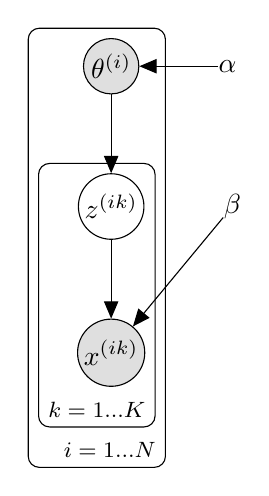
\begin{tikzpicture}[node distance = 1.5cm]
			\node[obs] (x) {$x^{(ik)}$}; 
			
			\node[latent, above=of x] (z) {$z^{(ik)}$}; 
			
			\node[obs, above=of z] (d) {$\theta^{(i)}$}; 
			
			\node[const, right=of d] (a) {$\alpha$} ;
			\node[const, right=of z] (th) {$\beta$} ;
			
			\edge {a} {d};
			\edge {z} {x};
			\edge {d} {z};
			\edge {th} {x};
			
			
			\plate {xz} {(x)(z)} {$k = 1...K$};
			\plate {xzd} {(x)(z)(d)(xz)} {$i = 1...N$};
			
			\end{tikzpicture}
		\end{minipage}%
		\begin{minipage}{0.50\textwidth}
			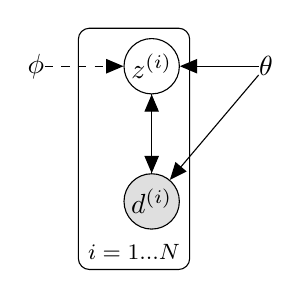
\begin{tikzpicture}[node distance = 1.5cm]
			\node[obs] (d) {$d^{(i)}$};
			
			\node[latent, above=of d] (z) {$z^{(i)}$};
			
			\node[const, right=of z] (th) {$\theta$} ;
			\node[const, left=of z] (ph) {$\phi$};
			
			
			\edge {z} {d};
			\edge {th} {z};
			\edge {th} {d};
			\edge [dashed,bend left] {d} {z}
			\edge [dashed] {ph} {z}
			
			
			
			\plate {zd} {(z)(d)} {$i = 1...N$};
			
			\end{tikzpicture}
		\end{minipage}
		
		\vspace{5mm}
		
		\hspace{15mm} LDA \hspace{25mm} SGVB Topic Model
	\end{frame}
	
	\begin{frame}
		\frametitle{So, whats different?}
		\begin{itemize}
			\item SGVB allows for powerful neural nets instead of linear.
			\item Document-level, as opposed to word-level latent variables places each document in relation to others.
			\item Continuous latent variables could lead to a traversible, smooth latent (topic) space, which can be more informative.
			\item SGVB allows for many different architectures and extensions, and scales well.
		\end{itemize}
	\end{frame}
	
	\begin{frame}
		\frametitle{Using a Graph Convolutional Encoder}
		We can see the word-topic occurrence matrix as a (sparse) graph, and use a GCE\footnote{Kipf, Thomas N., and Max Welling. "Semi-Supervised Classification with Graph Convolutional Networks." (2016).}. The first layer of our encoder $P(z|x)$ then becomes: 
		
		\begin{align}
		H = \text{ReLu}(\bar{D}^{-\frac{1}{2}}\bar{A}\bar{D}^{-\frac{1}{2}}XW)
		\end{align}
		
		For batch optimization to be viable, we need to alter the matrix $X$ somewhat.
	\end{frame}
		
	
	
\end{document}